%% The following is a directive for TeXShop to indicate the main file
%%!TEX root = Thesis_Driver.tex
\graphicspath{{./Figures/}}
\chapter{Cooperative Magnetic Inversion (CMI)}
\label{ch:Chap5_Cooperative_Mag_Inversion_CMI}

In Chapter \ref{ch:Chap3_Inverse}, I reviewed three magnetic inversion algorithms introduced in the literature. 
The magnetic susceptibility inversion is robust and computationally cheap, but it runs into limitations whenever the direction of magnetization is not parallel to the inducing field. 
The more general Magnetic Vector Inversion (MVI) can handle any orientation of magnetization by solving directly for the magnetization vector. 
This comes at the cost of increasing the number of unknowns in our large under-determined system of equations.
The $l_2$-norm regularization yields smooth solutions that are often too complex for direct geological interpretation.
Lastly, the inversion of magnetic amplitude data can provide a good estimate of the location and strength of magnetized bodies. 
The method is less sensitive to the orientation of magnetization than an inversion carried out with an assumed direction of magnetization.
The main complication for amplitude inversion is in computing amplitude data from the observed TMI, either via Fourier transform or by the equivalent-source. The inverse problem is also non-linear with respect to the model, which increases the computational cost and is less stable. 

While all of the above inversion methods have strength and weaknesses, they each bring complementary information.
The susceptibility inversion can be used to rapidly compute an equivalent-source layer and to generate amplitude data.
The amplitude data can then be fed into the amplitude inversion to locate magnetic anomalies.
In turn, imposing a geometric constraint on the MVI can greatly reduce the non-uniqueness of the problem. 
All three algorithms share variations of the same system of equations. This is beneficial as calcuations for the sensitivity matrix can be stored and repurposed at each step.

In this chapter, I introduce a Cooperative Magnetic Inversion (CMI) method, which combines the equivalent-source, amplitude inversion and MVI method into a single inversion algorithm. 
Using the S-IRLS method from Chapter~\ref{ch:Chap4_Mixed_Lpnorm_Regularization}, I impose a sparsity constraint on the model and model gradients to further reduce the solution space.
From an imaging stand point, compact and well defined magnetic anomalies can simplify the geological interpretation.
From a practical aspect, having an algorithm that can manage all three codes reduces the number of manual steps that were previously required from the user. 

\section{Methodology}
In Chapter \ref{ch:Chap3_Inverse}, I inverted a synthetic model with complicated magnetization orientations. 
The model recovered from the MVI inversion was smooth with poor recovery of the arc anomaly (Fig.~\ref{fig:3D_Inv_l2l2_model_TMVI}).
Using the CMI algorithm, I re-invert the synthetic example using an $l_2$-norm regularization. 
I will here breakdown each step of the CMI algorithm, but I want to emphasize that the entire process is automated and can all be done as a single workflow.
I divide the algorithm in three parts as shown in Figure \ref{fig:Advanced_Mag_Inversion_Algo} in schematic form.

 \begin{figure}[h!]
\centering
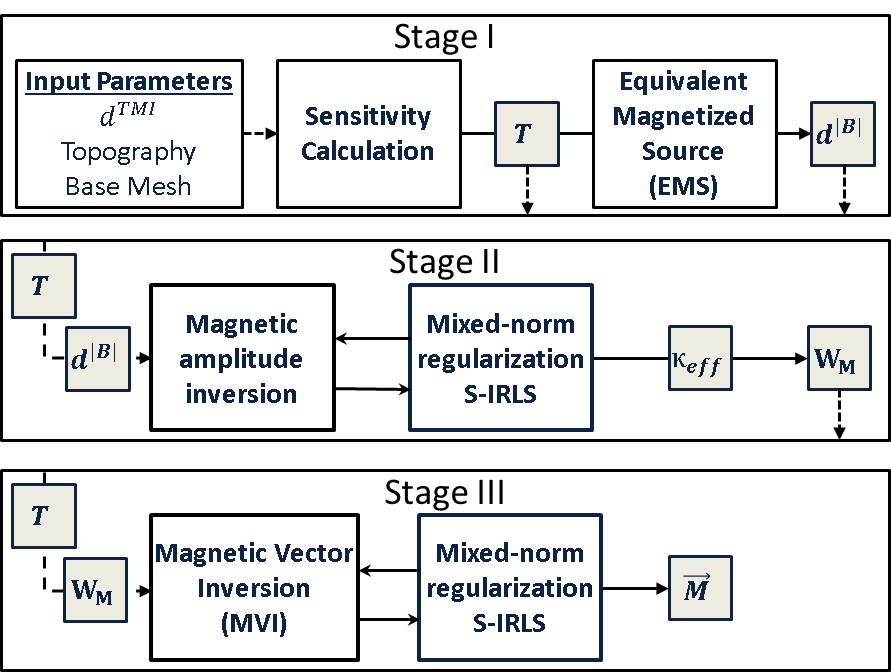
\includegraphics[scale=0.6]{Advanced_Mag_Inversion_Algo.png}
\caption{ Schematic representation of the Cooperative Magnetic Inversion (CMI) algorithm. Input and output parameters are indicated by a dash arrow.}
\label{fig:Advanced_Mag_Inversion_Algo}
\end{figure}

Stage I of the algorithm is mainly a data preparation step, ahead of the amplitude inversion and MVI.
As in other inversion methods, the algorithm requires TMA data and a mesh.
The algorithm computes the large system of equations needed for sensitivity calculations as defined by \ref{Tensor_T}.
Following the sensitivity calculations, the algorithm proceeds with an equivalent-source layer inversion as described in Section\ref{EQS}.
Figure~\ref{fig:3D_EQS_CMI} presents the inverted effective susceptibility layer and predicted data at the station locations.
Amplitude data are saved and passed on to Stage II.
\begin{figure}[p]
\centering
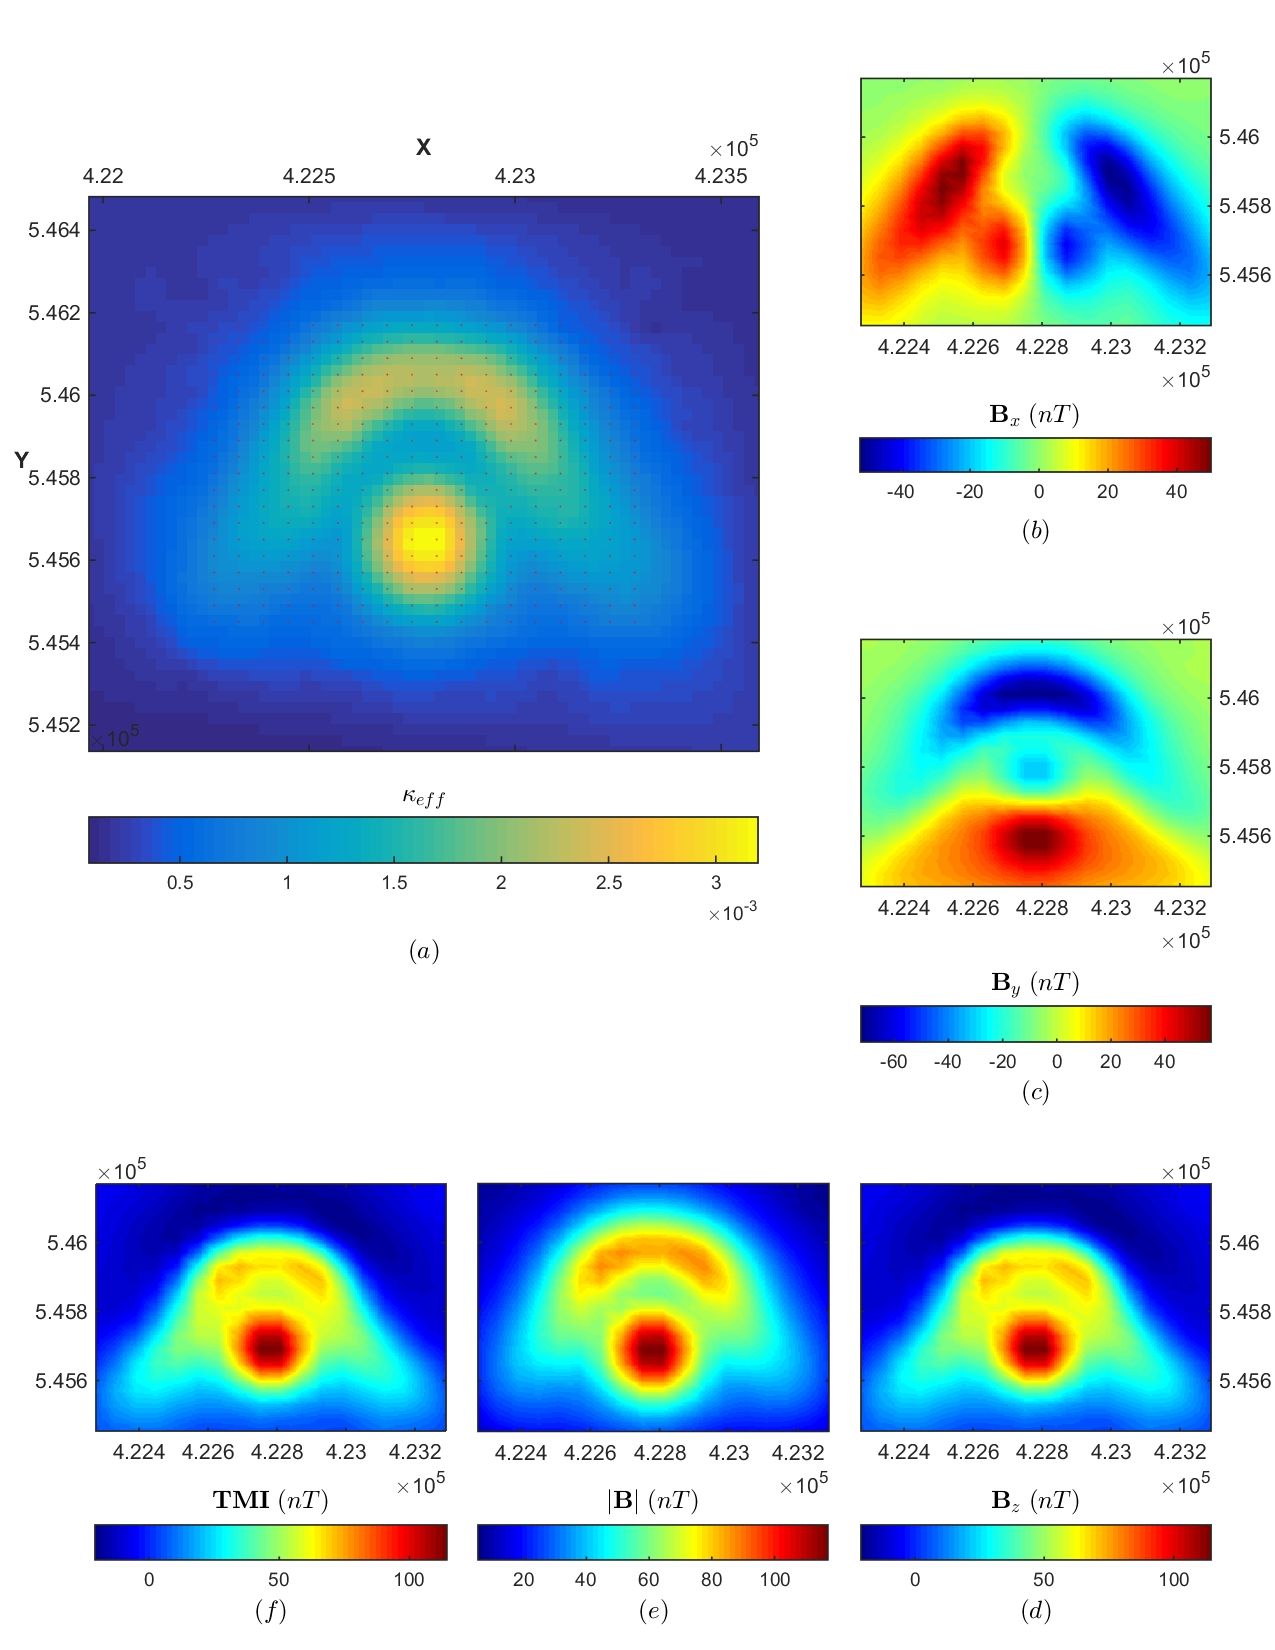
\includegraphics[scale=0.55]{3D_EQS_CMI.pdf}
\caption{ (a) Inverted equivalent-source layer and (b-f) predicted $\hat x$, $\hat y$, $\hat z$-component, TMI and magnetic amplitude data for the synthetic model.}
\label{fig:3D_EQS_CMI}
\end{figure}

In Stage II, the algorithm proceeds with the amplitude inversion from Section~\ref{MAI}.
Figure~\ref{fig:3D_Inv_l2l2_CMI_kEff} shows the recovered smooth effective susceptibility model.
The recovered effective susceptibility model is then converted to sensitivity weighting matrix such that:
\begin{equation}\label{W_M}
{W}_{m_{ii}} =  {\Big[\frac{\kappa_{e_i} *0.9 }{max(\kappa_{e})} + 0.01\Big]}^{-1}  \;,
\end{equation} 
 where $\mathbf{W}_m \in \mathbb{R}^{nc \times nc}$ is a diagonal matrix of the normalized effective susceptibilities $\kappa_{e}$. A small number (1e-2) is added to assure that all values are between [1 100].
 This type of re-scaling was determined empirically to be robust. 
The sensitivity weighting matrix is saved and passed on to the MVI inversion.

\begin{figure}[h!]
\centering
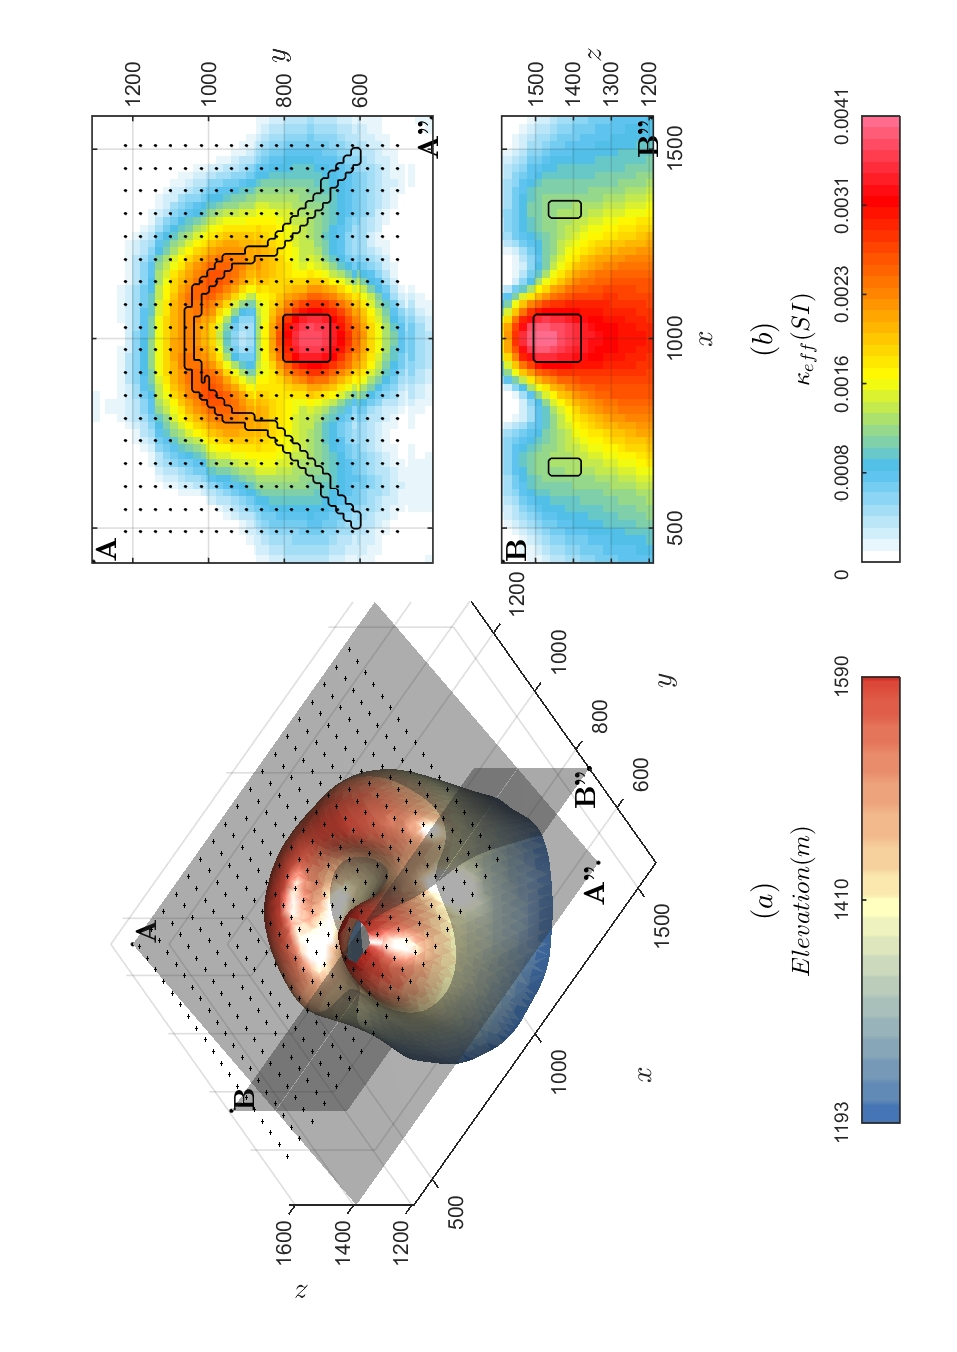
\includegraphics[scale=0.52, angle =270]{3D_Inv_l2l2_model_kEff.pdf}
\caption{ (a) Iso-surface (0.002 SI) and (b) sections through the recovered effective susceptibility model. This effective susceptibility model is used to construct a weighting matrix to constrain the MVI.}
\label{fig:3D_Inv_l2l2_CMI_kEff}
\end{figure}
\begin{figure}[h!]
\centering
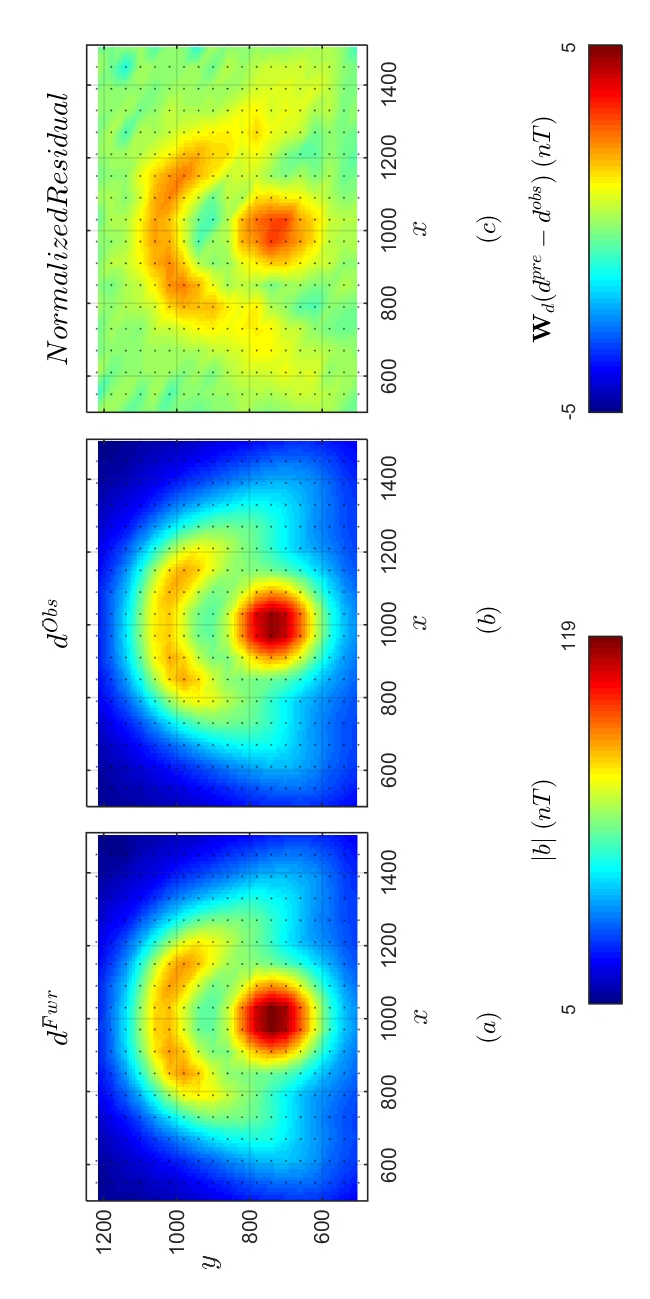
\includegraphics[scale=0.52, angle =270]{3D_Inv_l2l2_pred_kEff.pdf}
\caption{Comparison between (a) observed and (b) predicted data from the recovered effective susceptibility model. The inversion can predict most of the data within one standard deviation.}
\label{fig:3D_Inv_l2l2_pred_kEff}
\end{figure}

In Stage III, the regularization function is pre-multiplied by the effective susceptibility weighting calculated in \ref{W_M}.
The model objective function becomes:
\begin{equation} \label{eq:S-IRLS_CMI}
\begin{aligned}
\phi(m) =  \phi_d + \beta \gamma^{(k)} \Big [ {\|\mathbf{W}_m\; \mathbf{W}_s\;  \mathbf{\hat R}_s \;( \mathbf{m - m^{ref}})\|}^2_2  + \sum_{i = x,y,z}  {\| \mathbf{W}_m\;  \mathbf{W}_i \;  \mathbf{\hat R}_i  \; \mathbf{G}_i \; \mathbf{m}\|}^2_2  \Big ]\;.
\end{aligned}
  \end{equation}
 The model weighting matrix $\mathbf{W}_m$ imposes a high penalty on cells that received low effective susceptibility from the amplitude inversion. 
 Figure \ref{fig:3D_Inv_l2l2_model_AMI} presents the inverted model after reaching the target data misfit. The added information from the amplitude inversion greatly improves the solution over the MVI alone. Although still smoothly varying, the inversion manages to separate the arc and the block anomaly, while also recovering the orientation of magnetization.

\newpage
 \begin{figure}[h!]
\centering
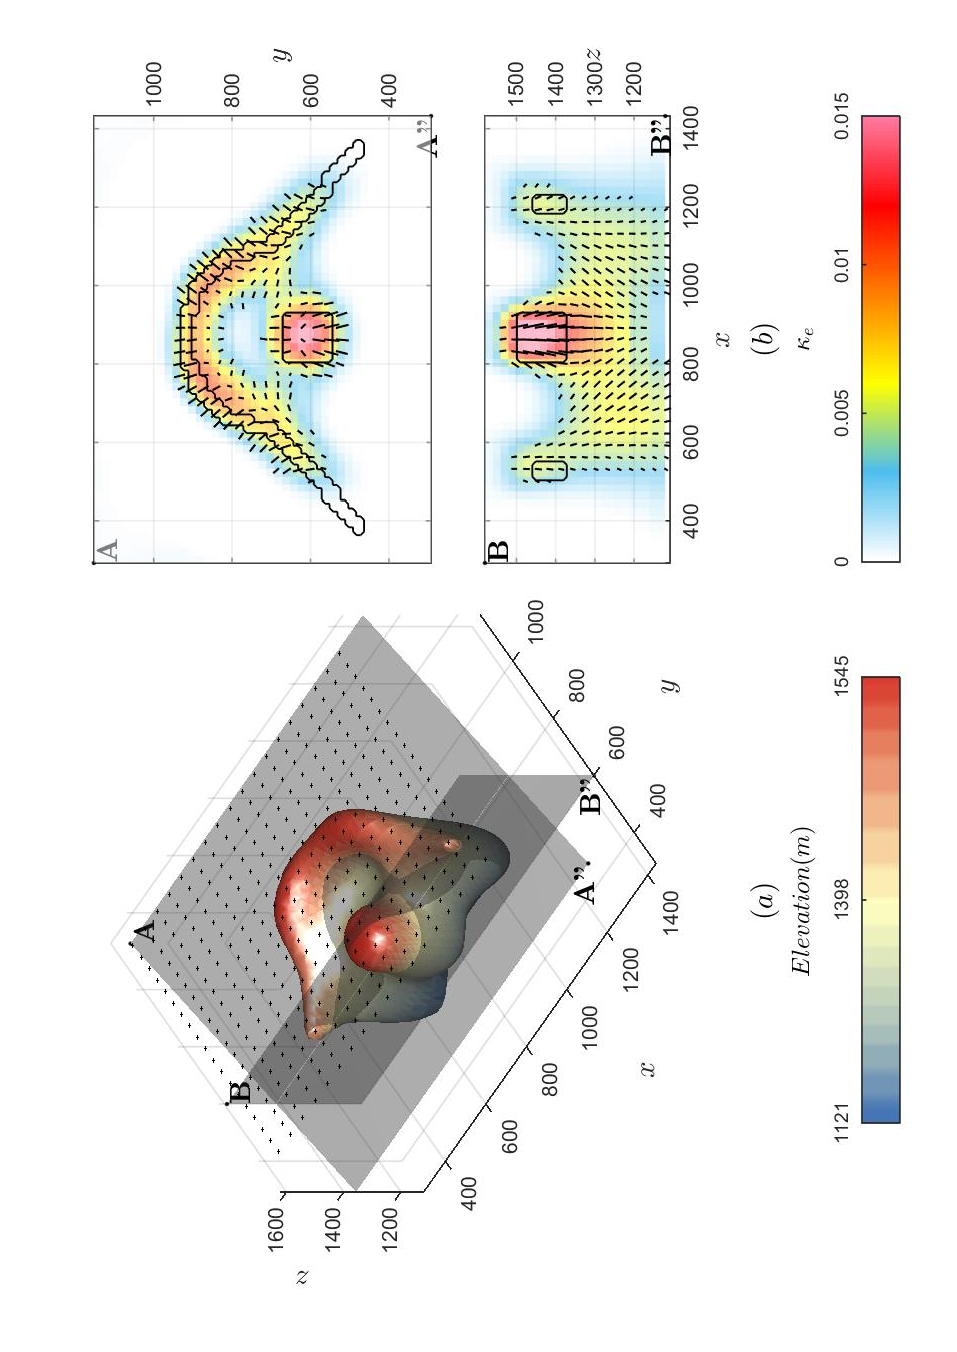
\includegraphics[scale=0.52, angle =270]{3D_Inv_l2l2_model_AMI.pdf}
\caption{ (a) Iso-surface (0.005 SI) and (b) sections through the recovered magnetization model from the CMI algorithm $(p = 2,\; q = 2)$ . The inversion recovers both the arc and the block anomaly as distinct objects.}
\label{fig:3D_Inv_l2l2_model_AMI}
\end{figure}
\begin{figure}[h!]
\centering
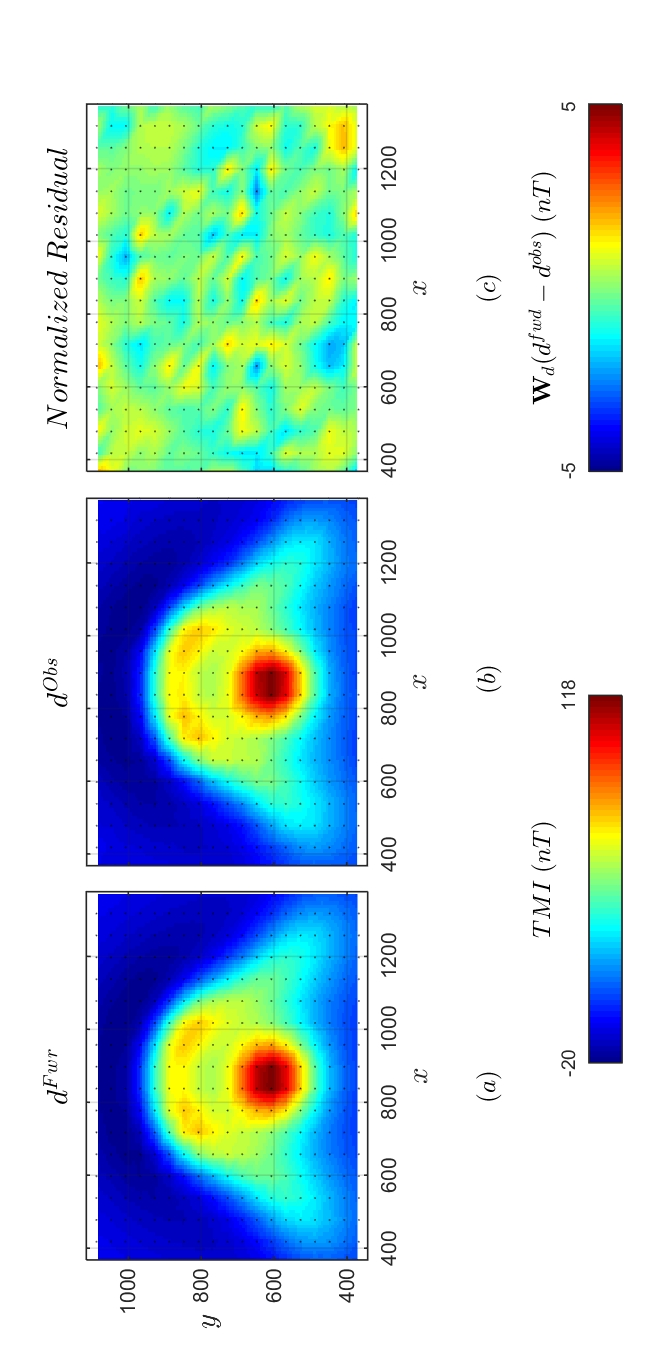
\includegraphics[scale=0.52, angle =270]{3D_Inv_l2l2_pred_AMI.pdf}
\caption{ Comparison between (a) observed and (b) predicted data from the recovered susceptibility model. (c) Normalized data residuals are within two standard deviations.}
\label{fig:3D_Inv_l2l2_pred_AMI}
\end{figure}

\newpage
\section{CMI with S-IRLS regularization}
As a final experiment I impose sparsity constraints on the amplitude inversion for $(p = 0,\; q = 1)$, in order to simplify the distribution of effective susceptibility. 
The goal is to get a simpler effective susceptibility model to further reduce the active space of the MVI algorithm. It is a $soft$ constraint on the solution as I do not impose $a\;priori$ information to individual cells, but rather a general constraint on the behavior of the solution. Figure~\ref{fig:3D_Inv_l0l1_CMI_kEff} presents the recovered model after convergence.

 The $l_p$-norm constraint considerably reduces the complexity of the model, although some artifacts remain at depth from the amplitude inversion.
 In Stage III, the compact effective susceptibility model is used to constrain the MVI result.
 Figure~\ref{fig:3D_Inv_l0l1_model_AMI} presents the final magnetization vector.
 The arc and the central block are recovered at the right location and effective susceptibility values are near the true model. 
 From a mineral exploration perspective, the model showed in \ref{fig:3D_Inv_l0l1_model_AMI}  would be easily interpreted.
 I note that most of the deep artifacts from the amplitude inversion have been removed. The final data residual is within one standard deviation, and no longer shows structure correlated with the magnetic anomaly.

\begin{figure}[h!]
\centering
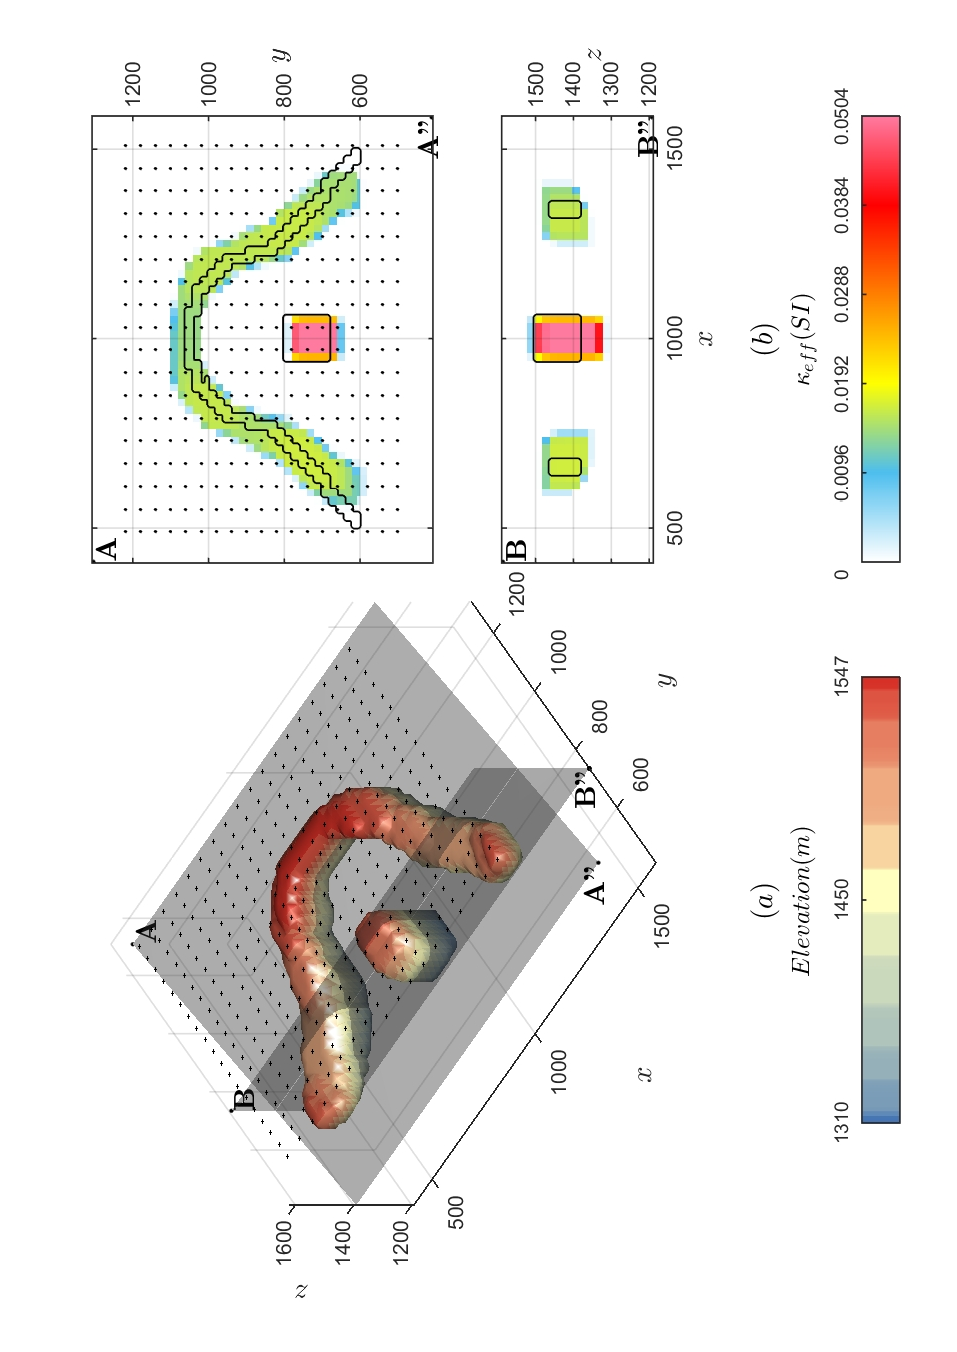
\includegraphics[scale=0.52, angle =270]{3D_Inv_l0l1_CMI_kEff.pdf}
\caption{ (a) Iso-surface (0.01 SI) and (b) sections through the recovered effective susceptibility model from the amplitude inversion with sparsity constraint applied $(p = 0,\; q = 1)$. The $l_p$-norm constraint considerably reduces the complexity of the model, although the model is still stretched vertically.}
\label{fig:3D_Inv_l0l1_CMI_kEff}
\end{figure}
\begin{figure}[h!]
\centering
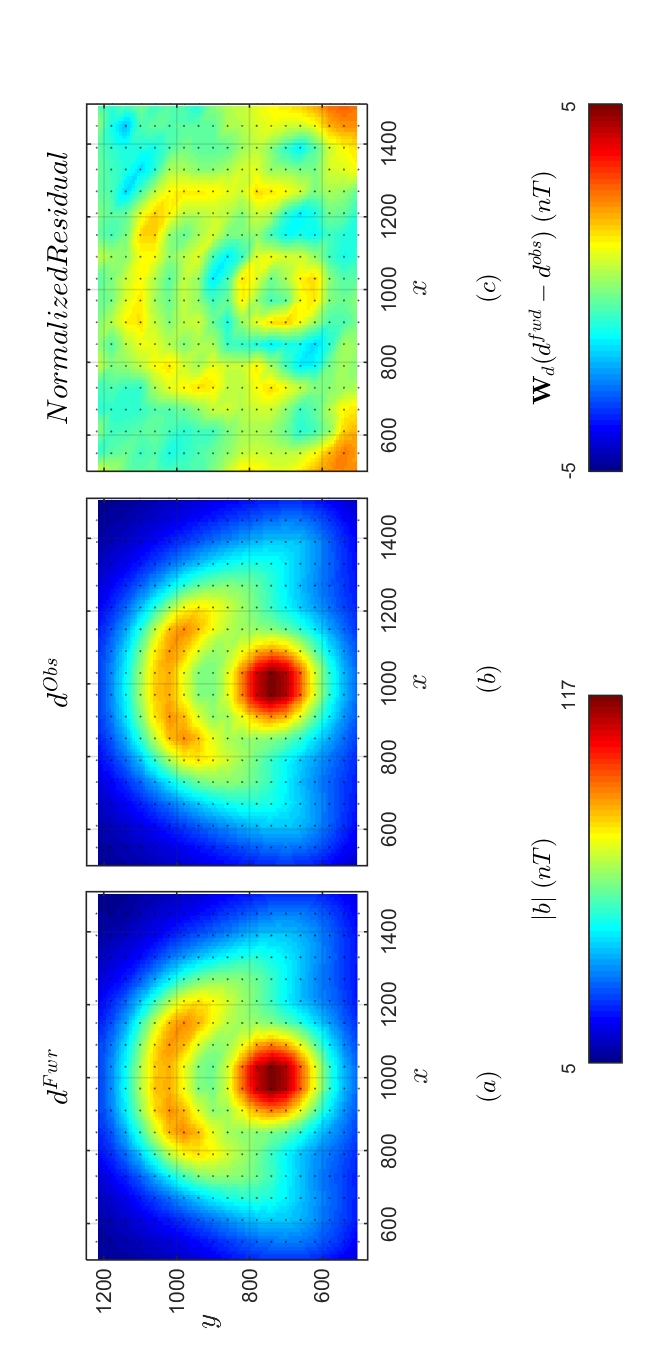
\includegraphics[scale=0.52, angle =270]{3D_Inv_l0l1_CMI_pred_kEff.pdf}
\caption{Comparison between (a) observed and (b) predicted amplitude data from the recovered compact effective susceptibility model $(p = 0,\; q = 1)$. (c) Normalized data residuals are within two standard deviations.}
\label{fig:3D_Inv_l0l1_CMI_pred_kEff}
\end{figure}

\begin{figure}[h!]
\centering
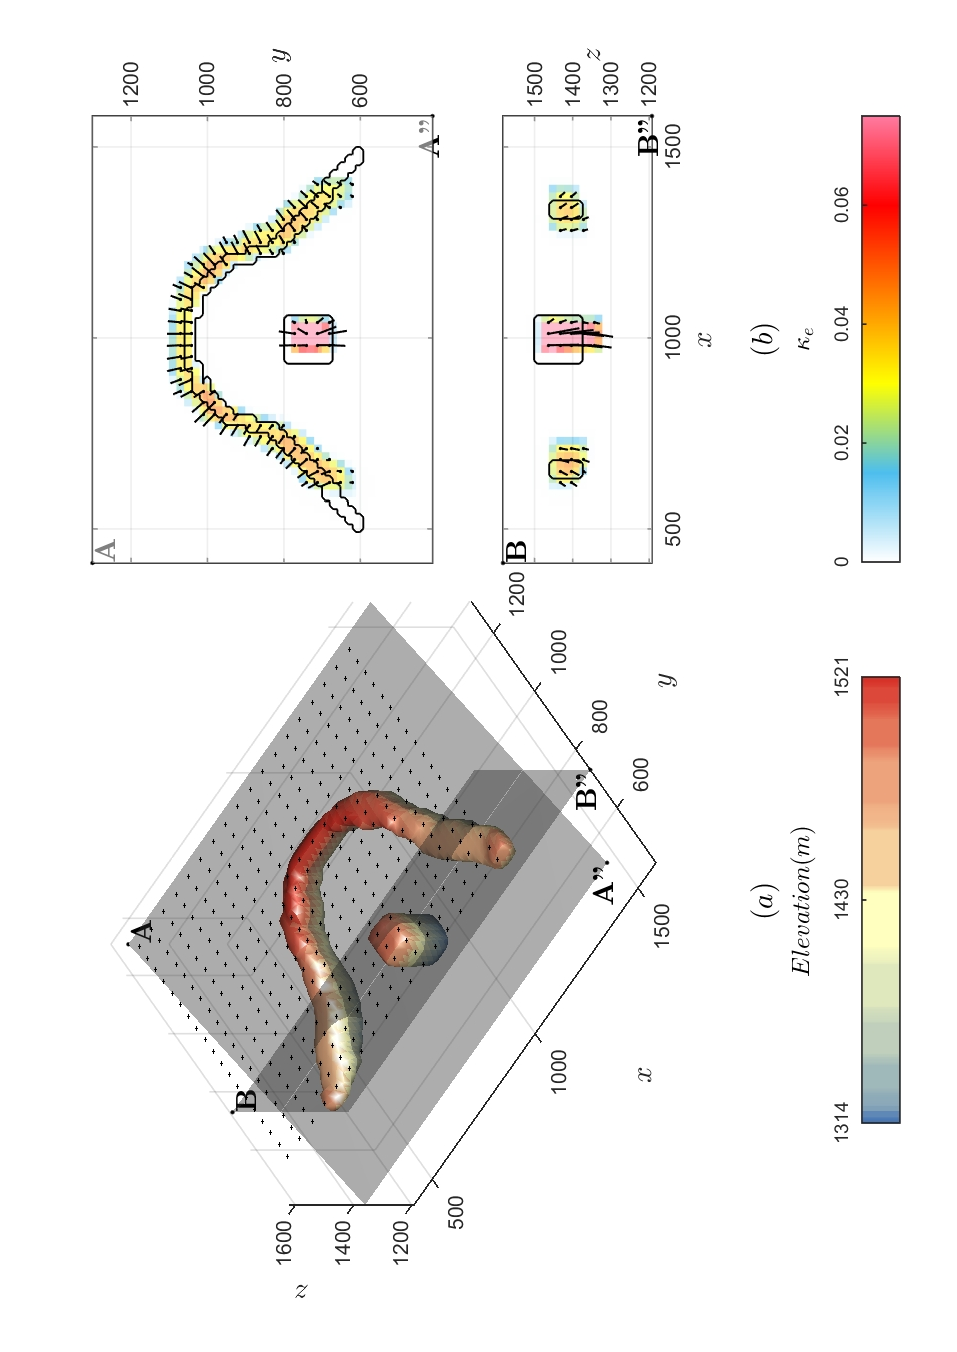
\includegraphics[scale=0.52, angle =270]{3D_Inv_l0l1_model_AMI.pdf}
\caption{ (a) Iso-surface (0.01 SI) and (b) sections through the recovered magnetization model from the CMI algorithm. Compact norms $(p = 0,\; q = 2)$ were applied during the amplitude inversion. The $l_p$-norm constraint considerably reduces the complexity of the model.}
\label{fig:3D_Inv_l0l1_model_AMI}
\end{figure}
\begin{figure}[h!]
\centering
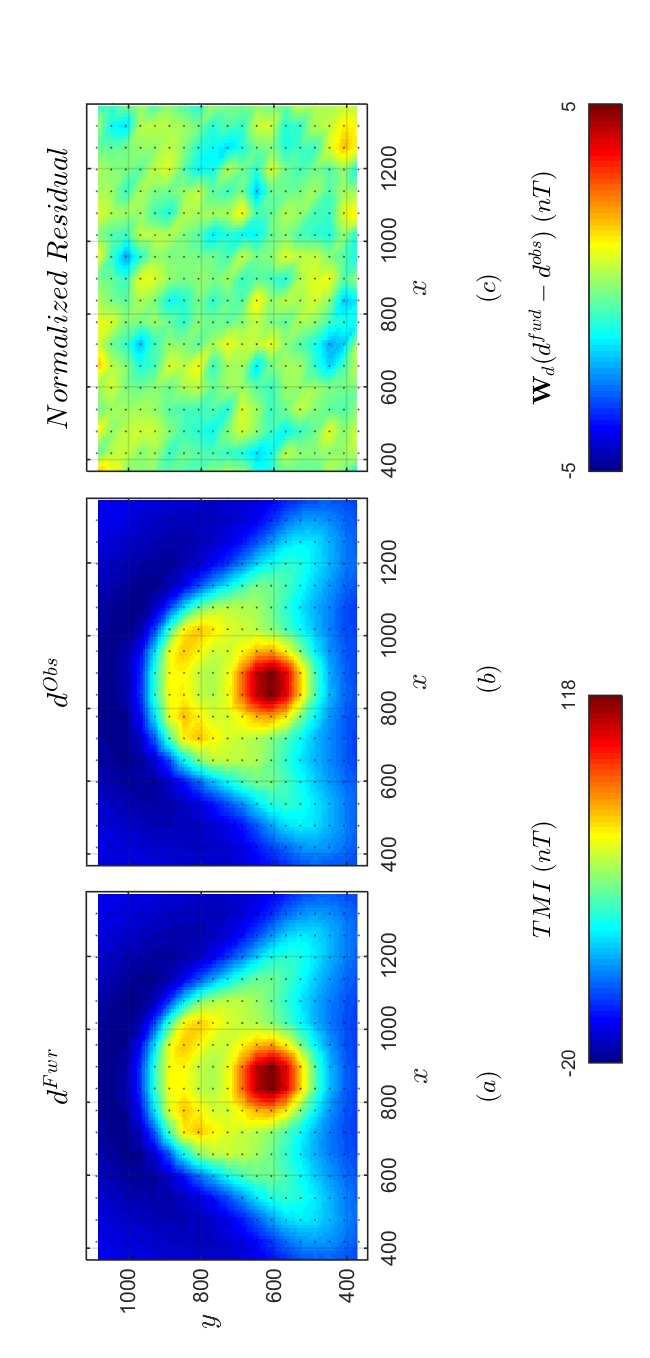
\includegraphics[scale=0.52, angle =270]{3D_Inv_l0l1_pred_AMI.pdf}
\caption{ Comparison between (a) observed and (b) predicted data from the recovered magnetization CMI model. (c) Normalized data residuals are within two standard deviations. Correlated residuals are no longer seen.}
\label{fig:3D_Inv_l2l2_pred_AMI}
\end{figure}

 \section{Conclusion}   
In this chapter, I implemented a Cooperative Magnetic Inversion for the inversion of magnetization vectors.
The algorithm ties together three inversion algorithms previously introduced in the literature: the magnetic susceptibility, magnetic amplitude and MVI.
The recovered vector magnetization models are simpler and more representative of the true solution. 
The inversion process is automated, hence reducing the overall work required, both numerically and from the end-user. 
    


\endinput

